\lhead{\textbf{Basic Algorithms, Fall 2024 \\ CSCI-UA.0310-001}}
\chead{\Large{\textbf{Homework 5}}}
\def\lc{\left\lceil}   
\def\rc{\right\rceil}
\rhead{\textbf{Instructor: Rotem Oshman \\
Name: Ishan Pranav}}
\runningheadrule
\firstpageheadrule
\cfoot{}
\stepcounter{subsection}
\subsection*{References}
Collaborated with Crystal Huang.

\subsection{Fast sorting}

\begin{enumerate}
    \item Assume you are given an array of $n$ integers in the range
    $\{1,\ldots, (\log n)^{\log n}\}$. Show how to sort this array in time
    $O(n \log\!\log n)$.

\begin{solution}

\end{solution}


    \item Assume you are given an array of $n$ integers with many
    duplicates, so that you know that there are at most $\log n$
    distinct elements in the array. Show how to sort this array in time
    $O(n)$ if you can use an arbitrary amount of memory, i.e., arrays of arbitrary sizes).
    \hint{Try to adapt the idea of counting sort by additionally keeping track of which elements exist in the array}

\begin{solution}   INSERT YOUR SOLUTION HERE   \end{solution}
\end{enumerate}





\subsection{Rod Cutting with Cost (4+4+2+4+1=15 points)}
Recall the Rod Cutting problem from the lecture: Suppose we have a rod of length $n$ inches and we also have an array of prices $P$, where $P[i]$ denotes the selling price (\$) of a piece that is $i$ inches long. Using dynamic programming (DP), one can efficiently find the maximal revenue obtained by cutting the rod and selling the individual pieces. 

Suppose now we have to pay a cost of \$1 per cut. Define the \emph{profit} we make as the revenue minus the total cost of cutting. We want an algorithm that finds a way to cut the rod that maximizes our \textbf{profit}. For example, if we have $P = (2,5,6,7)$ and $n=4$, then cutting it into two rods of length $2$ yields optimal profit $9=P[2]+P[2]-1$.

\begin{enumerate}
    \item Describe recursive formula $R(i)$ for the maximal profit when having a rod of length $i$. (You can use the values of $P$ inside your formula.) Do not forget the base case and justify the correctness of your formula. 
    \hint{How does this compare to the recursive formula for the basic rod-cutting problem?}
\begin{solution}   INSERT YOUR SOLUTION HERE   \end{solution}

    \item Implement your strategy using top-down DP with memoization.
\begin{solution}   INSERT YOUR SOLUTION HERE   \end{solution}
\end{enumerate} 

In the following, we want to implement a solution using \emph{bottom-up} DP, i.e., using an array to store the solutions rather than recursion.
For your DP algorithm, use the name $\textsc{MaxProfit}$ for the (potentially multi-dimensional) array which stores values of the subproblems.
\begin{enumerate}[resume]   
    \item Describe in words what $\textsc{MaxProfit}$ should be and state its dimension.
\begin{solution}   INSERT YOUR SOLUTION HERE   \end{solution}

    \item Implement your solution using bottom-up dynamic programming. 
\begin{solution}   INSERT YOUR SOLUTION HERE   \end{solution}

    \item Justify the run time of your algorithm to compute $\textsc{MaxProfit}$ as a big-$\Theta$ expression.
    
\begin{solution}   INSERT YOUR SOLUTION HERE   \end{solution}
\end{enumerate}



\subsection{Subset Sum (2+1+1+5+2=11 points)}
Let $A = [a_1, \ldots, a_n]$ be an array of $n$ natural numbers. Given a number $t \in \mathbb{N}$, we say $t$ is a \emph{subset sum} of $A$ if there is a \emph{subset of indices} $S \subseteq \{1,\ldots,n\}$ such that $\sum_{i \in S} a_i = t$. For example, if $A=[1,3,5,7]$ then $12$ is a subset sum of $A$ since $5+7=12$, but $2$ is not. (Note that each value can only be included in the sum at most once.)

We want to design an algorithm that determines whether a given number $t \in \mathbb{N}$ is a subset sum of $A$. Specifically, when given $A = [a_1,\ldots,a_n]$ and $t \in \mathbb{N}$ as input, the algorithm should output $1$ if $t$ is a subset sum of $A$, and $0$ otherwise.
We will use (bottom-up) dynamic programming with a two-dimensional array to solve this problem. The subproblem in your DP algorithm should be $\textsc{SubsetSum}$, which is defined as
\begin{align*}
\textsc{SubsetSum}[i][t] = 
\begin{cases} 
    1 &\text{ if $t$ is a subset sum of the first $i$ elements $A_{1:i}=[a_1,\ldots,a_i]$,} \\
    0 &\text{ otherwise.}
\end{cases}
\end{align*}

Also, let us define $M = \sum_{i=1}^n a_i$, which is the sum of all numbers in $A$. The quantity $M$ may appear in the size of the DP array and the run-time of your algorithm.

\begin{enumerate}
    \item Suppose $A=[2,1,3]$. Fill out the following table for $A$. Note that we define the sum over the empty set to be $0$. The pre-filled entries in the top left corner correspond to $\textsc{SubsetSum}[0][0]=1$ and $\textsc{SubsetSum}[0][1]=0$.
    \begin{table}[H]
        \centering
        \captionsetup{width=.7\linewidth}
        \begin{tabular}{|c|c|c|c|c|c|c|c|}
            \hline
            \backslashbox{$i$}{$t$} & 0 & 1 & 2 & 3 & 4 & 5 & 6\\
            \hline
            0 & 1 & 0 & \hspace{6ex} & \hspace{6ex} & \hspace{6ex} & \hspace{6ex} & \hspace{6ex} \\
            \hline
            1 & & \hspace{6ex} & \hspace{6ex} & \hspace{6ex} & \hspace{6ex} & \hspace{6ex} & \hspace{6ex} \\
            \hline
            2 & \hspace{6ex} & \hspace{6ex} & \hspace{6ex} & \hspace{6ex} & \hspace{6ex} & \hspace{6ex} & \hspace{6ex} \\
            \hline
            3 & \hspace{6ex} & \hspace{6ex} & \hspace{6ex} & \hspace{6ex} & \hspace{6ex} & \hspace{6ex} & \hspace{6ex} \\
            \hline
        \end{tabular}
        \caption{Fill in the entries for $\textsc{SubsetSum}[i][t]$.}
        \label{tab:subset-sum}
    \end{table}

    
    \item In general, what is the size of the DP array containing values for $\textsc{SubsetSum}$? \hint{What is the largest number you could even conceivably obtain as a subset sum of $A$? You may want to make use of $M$ for your expression.}
\begin{solution}   INSERT YOUR SOLUTION HERE   \end{solution}
    
    \item State the base cases for $i=0$, i.e., state all the values for $i=0$.
\begin{solution}   INSERT YOUR SOLUTION HERE   \end{solution}

    \item Give and justify the recurrence $\textsc{SubsetSum}$ should satisfy. \hint{Given inputs $i$ and $t$, we can either use the $i$-th element $a_i$ or not use it in the subset sum for $t$. If we use $a_i$, then the remaining subset sum is $t-a_i$ which is less than $t$.}
\begin{solution}   INSERT YOUR SOLUTION HERE   \end{solution}
    
    \item For a bottom-up DP implementation, in which order do you have to fill the two-dimensional table for your algorithm to work? Should you fill it row by row or column by column? And within each row/column, does the order matter? \hint{You must make sure that only values already filled in are read by the algorithm.}
\begin{solution}   INSERT YOUR SOLUTION HERE   \end{solution}
\end{enumerate}


\subsection*{Honors Question 1: Fast Sorting}

Recall Question~1.2. Solve the question in time $O(n \log\!\log n)$ but using only $O(n)$ space. Only use data structures introduced in the lecture; do not use hash tables. \hint{Consider using ideas from Insertion Sort to adapt your solution from the previous part.}

\begin{solution}   INSERT YOUR SOLUTION HERE   \end{solution}



\subsection*{Honors Question: Tiling}
{\bf (**)} Given an $m\times n$ size rectangle, we wish to divide it into non-overlapping square pieces, using the least possible number of pieces. For example a $4\times 5$ rectangle needs at least $5$ pieces: a big $4\times 4$ square and $4$ small $1\times 1$ squares.


\begin{figure}[!ht]
    \centering
    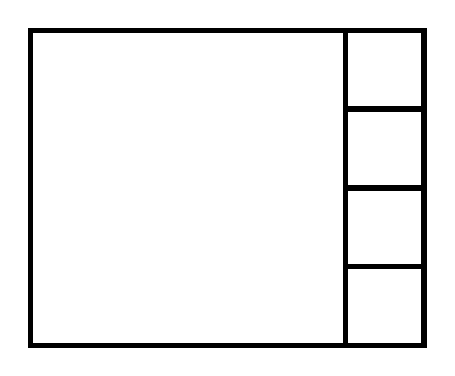
\begin{tikzpicture}
    \draw[line width=2pt] (0,0) rectangle (5,4);
    \draw[line width=2pt] (4,0) -- (4,4);
    \draw[line width=2pt] (4,1) -- (5,1);
    \draw[line width=2pt] (4,2) -- (5,2);
    \draw[line width=2pt] (4,3) -- (5,3);  
    \end{tikzpicture}
    \caption{Dividing up a $4\times 5$ rectangle using $5$ squares}
\end{figure}

We might try to solve this using the idea of trying to cut the $n\times m$ size rectangle into two pieces either by a vertical or a horizontal cut. The following pseudo-code tries all possible horizontal and vertical cuts and picks the best case out of these.
\begin{algorithm}[]
\begin{algorithmic}
\STATE $\textsc{MinTilings}(m,n)$:
\IF{$m==n$}
\RETURN $1$.
\ENDIF
\STATE $H_{min} = \textsc{INT}_\textsc{MAX}$.
\STATE $V_{min} = \textsc{INT}_\textsc{MAX}$.
\FOR{$i=1$ \TO $\lfloor m/2 \rfloor$}
\STATE  $H_{\min} = \min(H_{\min},\textsc{MinTilings}(i,n)+\textsc{MinTilings}(m-i,n))$.
\ENDFOR
\FOR{$j=1$ \TO $\lfloor n/2 \rfloor$}
\STATE  $V_{min} = \min(V_{\min},\textsc{MinTilings}(m,j)+\textsc{MinTilings}(m,n-j))$.
\ENDFOR
\RETURN $\min(H_{\min},V_{\min})$.
\end{algorithmic}
\end{algorithm}
\newline
Use dynamic programming to improve this recursive method by avoiding re-computation for sub-problems that have already been solved. What is the running time of your algorithm?

Does this approach work to find the \emph{optimal} tiling? Why or why not? (Hint: Consider the figure below)

\begin{figure}[!ht]
    \centering
    \scalebox{0.67}{
    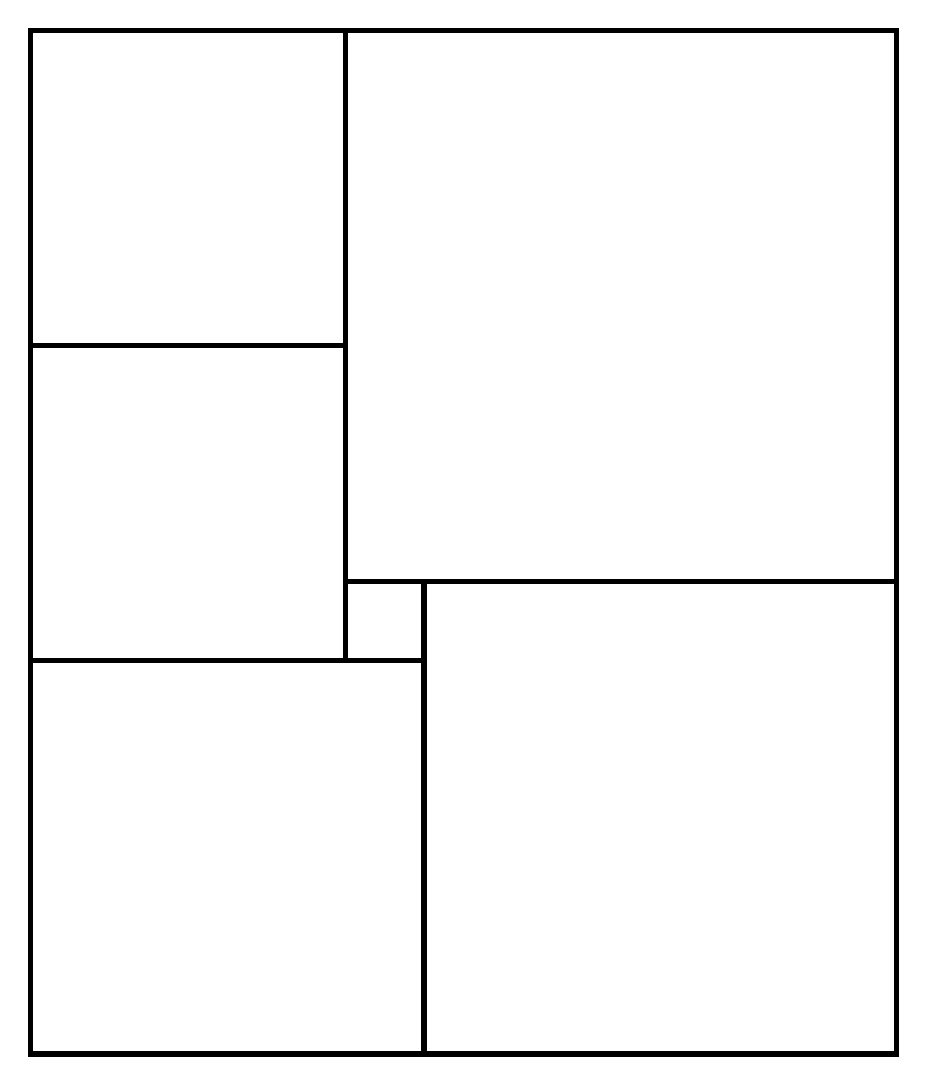
\begin{tikzpicture}
    \draw[line width=2pt] (0,0) rectangle (11,13);
    \draw[line width=2pt] (5,0) -- (5,6);
    \draw[line width=2pt] (0,5) -- (5,5);   
    \draw[line width=2pt] (4,5) -- (4,13);   
    \draw[line width=2pt] (0,9) -- (4,9);     
    \draw[line width=2pt] (4,6) -- (11,6);   
    \end{tikzpicture}
    }
    \caption{Dividing up a $11\times 13$ rectangle using $6$ squares (two $4\times 4$ squares and one each of $1\times 1$, $5\times 5$, $6\times 6$ and $7\times 7$ squares)}
\end{figure}
